

\chapter{Channels}

\par{} Communications between either a client application and a
service-- and possibly between two client applications via a service--
are handled over a service channel. A service channel is the logical
encapsulation of bidirectional data over an existing sametime
session. Creating or using a channel does not require an additional
TCP connection.

\par{} The sametime protocol defines four specific messages as key in
the operation of a channel; channel create, channel accept, channel
send, and channel close.

\par{} Channels are tagged by a 32-bit identifier, which must be
unique only within that session. Channel identifiers may be re-used,
and may be utilized in any (or no) order. The only constraint in
generating a channel id is that the most-significant bit must be unset
for locally-initiated channels, and set for remotely-initiated
channels. For example,

\begin{itemize}
\item \code{0x80000042} would be a remote channel, which the local
session would need to accept.
\item \code{0x00000042} would be a local channel, which the target
service would need to accept.
\end{itemize}

\par{} Whether a channel is local or remote is relative. Therefore,
the channel id will never be identical for either end of the channel.


\section{Channel Creation}

\begin{figure}[!h]
  \begin{center}
    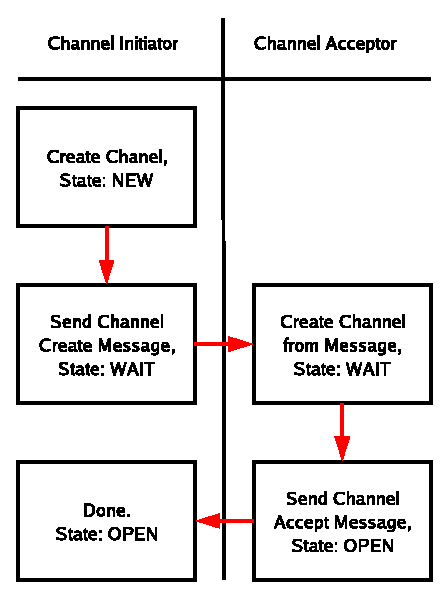
\includegraphics{diagrams/chan_create.eps}
  \end{center}
  \caption{Creation of a Channel}
  \label{chan_create}
\end{figure}

\begin{figure}[!h]
  \begin{center}
    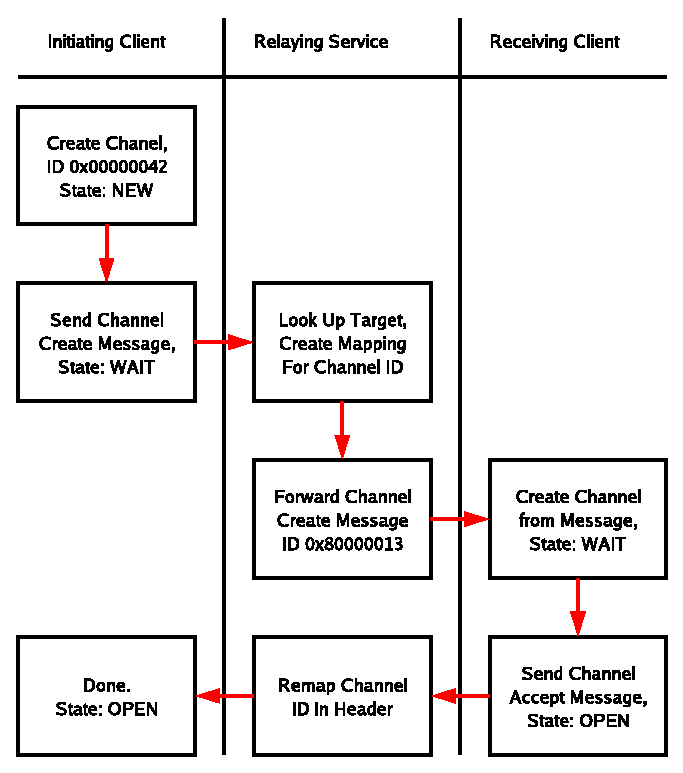
\includegraphics{diagrams/chan_create_proxy.eps}
  \end{center}
  \caption{Creation of a Channel between Clients}
  \label{chan_create_proxy}
\end{figure}

\par{} Figure \ref{chan_create} provides a brief illustration of the
channel creation process, while figure \ref{chan_create_proxy}
illustrates how a service can facilitate client-to-client channels.


\section{Sending Data Over a Channel}
\par{} Then you can send data over it.


\section{Closing a Channel}
\par{} And then you close it.


\section{Zero Channel}
\par{} The zero-- or master-- channel is tagged with the channel
identifier \code{0x00} and does not need to be created as other
channels do-- it is available from the very beginning of a session. In
fact, it is over the zero channel that the Handshake, Login, and
Create Channel messages are sent. The only real reason for having the
zero channel exist at all is due to the fact that the channel
identifier is a required part of all message types.
